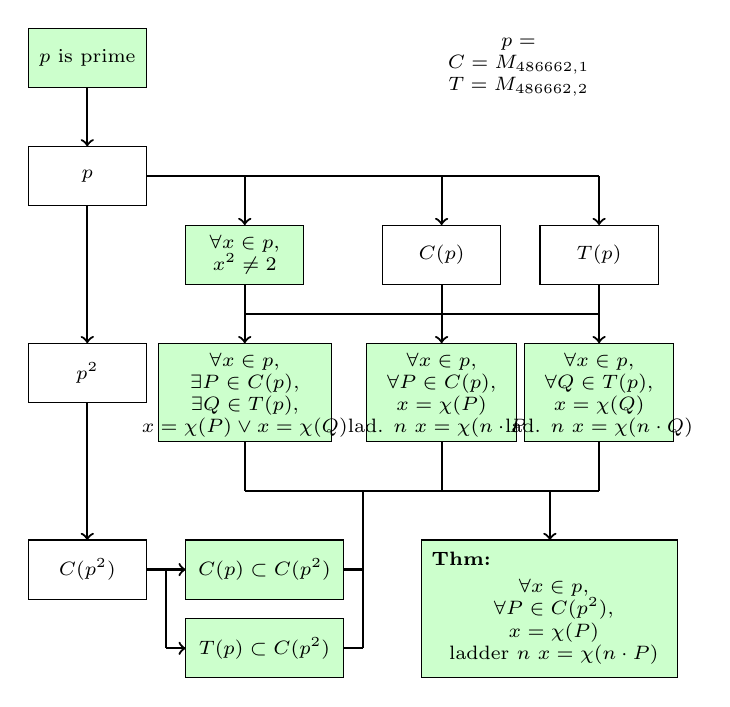
\begin{tikzpicture}[textstyle/.style={black, anchor= south west, align=center, minimum height=0.45cm, text centered, font=\scriptsize}]

  \draw (6.75,1.5) node[textstyle, anchor=north east] {$p = \p$\\$C = M_{486662,1}$\\$T = M_{486662,2}$\\};

  \begin{scope}[yshift=1.5 cm,xshift=-0.5 cm]
   \draw [fill=green!20] (0,0) -- (1.5,0) -- (1.5,-0.75) -- (0, -0.75) -- cycle;
   \draw (0.75,-0.375) node[textstyle, anchor=center] {$p$ is prime};
  \end{scope}

  \begin{scope}[yshift=0 cm,xshift=-0.5 cm]
   \draw[fill=white] (0,0) -- (1.5,0) -- (1.5,-0.75) -- (0, -0.75) -- cycle;
   \draw (0.75,-0.375) node[textstyle, anchor=center] {$\F{p}$};
  \end{scope}

  \begin{scope}[yshift=-1 cm,xshift=1.5 cm]
   \draw[fill=green!20] (0,0) -- (1.5,0) -- (1.5,-0.75) -- (0, -0.75) -- cycle;
   \draw (0.75,-0.375) node[textstyle, anchor=center] {$\forall x \in \F{p},$\\$x^2 \neq 2$};
  \end{scope}

  \begin{scope}[yshift=-1 cm,xshift=4 cm]
   \draw[fill=white] (0,0) -- (1.5,0) -- (1.5,-0.75) -- (0, -0.75) -- cycle;
   \draw (0.75,-0.375) node[textstyle, anchor=center] {$C(\F{p})$};
  \end{scope}

  \begin{scope}[yshift=-1 cm,xshift=6 cm]
   \draw[fill=white] (0,0) -- (1.5,0) -- (1.5,-0.75) -- (0, -0.75) -- cycle;
   \draw (0.75,-0.375) node[textstyle, anchor=center] {$T(\F{p})$};
  \end{scope}

  \path [thick, double, ->] (0.25,0.75) edge  [out=-90, in=90] (0.25,0);
  \path [thick, double]     (1,-0.375) edge  [out=0, in=180] (6.75,-0.375);
  \path [thick, double, ->] (2.25,-0.375) edge  [out=-90, in=90] (2.25,-1);
  \path [thick, double, ->] (4.75,-0.375) edge  [out=-90, in=90] (4.75,-1);
  \path [thick, double, ->] (6.75,-0.375) edge  [out=-90, in=90] (6.75,-1);


  \begin{scope}[yshift=-2.5 cm,xshift=1.5 cm]
   \draw[fill=green!20] (-0.35,0) -- (1.85,0) -- (1.85,-1.25) -- (-0.35, -1.25) -- cycle;
   \draw (0.75,0) node[textstyle, anchor=north] {$\forall x \in \F{p},$\\$\exists P \in C(\F{p}),$\\$\exists Q \in T(\F{p})$,\\$x = \chi(P)\vee x = \chi(Q)$};
  \end{scope}

  \begin{scope}[yshift=-2.5 cm,xshift=4 cm]
   \draw[fill=green!20] (-0.20,0) -- (1.70,0) -- (1.70,-1.25) -- (-0.20, -1.25) -- cycle;
   \draw (0.75,0) node[textstyle, anchor=north] {$\forall x \in \F{p},$\\$\forall P \in C(\F{p}),$\\$x = \chi(P)\implies$\\lad. $n$ $x = \chi(n \cdot P)$};
  \end{scope}

  \begin{scope}[yshift=-2.5 cm,xshift=6 cm]
   \draw[fill=green!20] (-0.20,0) -- (1.70,0) -- (1.70,-1.25) -- (-0.20, -1.25) -- cycle;
   \draw (0.75,0) node[textstyle, anchor=north] {$\forall x \in \F{p},$\\$\forall Q \in T(\F{p}),$\\$x = \chi(Q)\implies$\\lad. $n$ $x = \chi(n \cdot Q)$};
  \end{scope}

  \path [thick, double]     (2.25,-2.125) edge  [out=0, in=180] (6.75,-2.125);
  \path [thick, double, ->] (2.25,-1.75) edge  [out=-90, in=90] (2.25,-2.5);
  \path [thick, double, ->] (4.75,-1.75) edge  [out=-90, in=90] (4.75,-2.5);
  \path [thick, double, ->] (6.75,-1.75) edge  [out=-90, in=90] (6.75,-2.5);

% F(p^2)

  \path [thick, double, ->] (0.25,-0.75) edge  [out=-90, in=90] (0.25,-2.5);

  \begin{scope}[yshift=-2.5 cm,xshift=-0.5 cm]
   \draw[fill=white] (0,0) -- (1.5,0) -- (1.5,-0.75) -- (0, -0.75) -- cycle;
   \draw (0.75,-0.375) node[textstyle, anchor=center] {$\F{p^2}$};
  \end{scope}

  \path [thick, double, ->] (0.25,-3.25) edge  [out=-90, in=90] (0.25,-5);

  % C(F(p^2))

  \begin{scope}[yshift=-5 cm,xshift=-0.5 cm]
   \draw[fill=white] (0,0) -- (1.5,0) -- (1.5,-0.75) -- (0, -0.75) -- cycle;
   \draw (0.75,-0.375) node[textstyle, anchor=center] {$C(\F{p^2})$};
  \end{scope}

  \begin{scope}[yshift=-5 cm,xshift=1.5 cm]
   \draw[fill=green!20] (0,0) -- (2,0) -- (2,-0.75) -- (0, -0.75) -- cycle;
   \draw (1,-0.375) node[textstyle, anchor=center] {$C(\F{p}) \subset C(\F{p^2})$};
  \end{scope}

  \begin{scope}[yshift=-6 cm,xshift=1.5 cm]
   \draw[fill=green!20] (0,0) -- (2,0) -- (2,-0.75) -- (0, -0.75) -- cycle;
   \draw (1,-0.375) node[textstyle, anchor=center] {$T(\F{p}) \subset C(\F{p^2})$};
  \end{scope}

  \path [thick, double, ->] (1,-5.375) edge [out=0, in=-180] (1.5,-5.375);
  \path [thick, double] (1.25,-5.375) edge [out=-90, in=90] (1.25,-6.375);
  \path [thick, double, ->] (1.25,-6.375) edge [out=0, in=-180] (1.5,-6.375);

  \begin{scope}[yshift=-5 cm,xshift=4.5 cm]
    \draw [fill=green!20] (0,0) -- (3.25,0) -- (3.25,-1.75) -- (0, -1.75) -- cycle;
    \draw (0,0) node[textstyle, anchor=north west] {\textbf{Thm:}};
    \draw (1.675,-0.375) node[textstyle, anchor=north] {$\forall x \in \F{p},$\\$\forall P \in C(\F{p^2}),$\\$x = \chi(P)\implies$\\ladder $n$ $x = \chi(n \cdot P)$};
  \end{scope}

  \path [thick, double]     (2.25,-4.375) edge  [out=0, in=180] (6.75,-4.375);
  \path [thick, double]     (2.25,-3.75) edge  [out=-90, in=90] (2.25,-4.375);
  \path [thick, double]     (4.75,-3.75) edge  [out=-90, in=90] (4.75,-4.375);
  \path [thick, double]     (6.75,-3.75) edge  [out=-90, in=90] (6.75,-4.375);

  \path [thick, double]     (3.5,-5.375) edge  [out=0, in=180] (3.75,-5.375);
  \path [thick, double]     (3.5,-6.375) edge  [out=0, in=180] (3.75,-6.375);
  \path [thick, double]     (3.75,-6.375) edge  [out=90, in=-90] (3.75,-4.375);

  \path [thick, double, ->] (6.125,-4.375) edge [out=-90, in=90] (6.125,-5);

\end{tikzpicture}
